\tikzset{every picture/.style={line width=0.75pt}} %set default line width to 0.75pt        

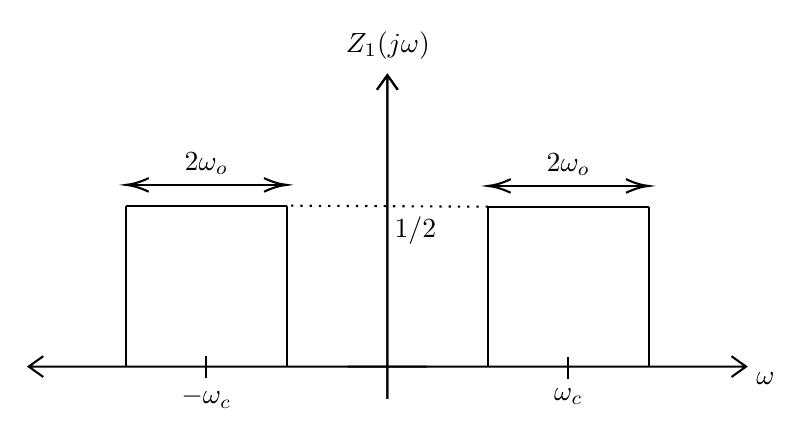
\begin{tikzpicture}[x=0.75pt,y=0.75pt,yscale=-1,xscale=1]
%uncomment if require: \path (0,300); %set diagram left start at 0, and has height of 300

%Shape: Axis 2D [id:dp4364414837639843] 
\draw  (301,209.4) -- (493,209.4)(320.2,69) -- (320.2,225) (486,204.4) -- (493,209.4) -- (486,214.4) (315.2,76) -- (320.2,69) -- (325.2,76)  ;
%Shape: Axis 2D [id:dp20109394216457532] 
\draw  (339.4,209.4) -- (147.4,209.4)(320.2,69) -- (320.2,225) (154.4,204.4) -- (147.4,209.4) -- (154.4,214.4) (325.2,76) -- (320.2,69) -- (315.2,76)  ;
%Straight Lines [id:da7559993359973315] 
\draw    (233,204.29) -- (233,214.71) ;
%Straight Lines [id:da21670318107864883] 
\draw    (407.4,204.8) -- (407.4,215.22) ;
%Straight Lines [id:da3439489556285271] 
\draw    (194.29,131.87) -- (194.29,209.29) ;
%Straight Lines [id:da19666501065127062] 
\draw  [dash pattern={on 0.84pt off 2.51pt}]  (368.69,132.38) -- (271.71,131.87) ;
%Straight Lines [id:da5487354351298724] 
\draw    (271.71,131.87) -- (194.29,131.87) ;
%Straight Lines [id:da1866677761933241] 
\draw    (271.71,131.87) -- (271.71,209.29) ;
%Straight Lines [id:da45800765996237425] 
\draw    (446.11,132.38) -- (368.69,132.38) ;
%Straight Lines [id:da07434960977090421] 
\draw    (368.69,132.38) -- (368.69,209.8) ;
%Straight Lines [id:da2890856974084346] 
\draw    (446.11,132.38) -- (446.11,209.8) ;
%Straight Lines [id:da34528122862725874] 
\draw    (196.29,121.87) -- (269.71,121.87) ;
\draw [shift={(271.71,121.87)}, rotate = 180] [color={rgb, 255:red, 0; green, 0; blue, 0 }  ][line width=0.75]    (10.93,-3.29) .. controls (6.95,-1.4) and (3.31,-0.3) .. (0,0) .. controls (3.31,0.3) and (6.95,1.4) .. (10.93,3.29)   ;
\draw [shift={(194.29,121.87)}, rotate = 0] [color={rgb, 255:red, 0; green, 0; blue, 0 }  ][line width=0.75]    (10.93,-3.29) .. controls (6.95,-1.4) and (3.31,-0.3) .. (0,0) .. controls (3.31,0.3) and (6.95,1.4) .. (10.93,3.29)   ;
%Straight Lines [id:da4595793235204215] 
\draw    (370.69,122.38) -- (444.11,122.38) ;
\draw [shift={(446.11,122.38)}, rotate = 180] [color={rgb, 255:red, 0; green, 0; blue, 0 }  ][line width=0.75]    (10.93,-3.29) .. controls (6.95,-1.4) and (3.31,-0.3) .. (0,0) .. controls (3.31,0.3) and (6.95,1.4) .. (10.93,3.29)   ;
\draw [shift={(368.69,122.38)}, rotate = 0] [color={rgb, 255:red, 0; green, 0; blue, 0 }  ][line width=0.75]    (10.93,-3.29) .. controls (6.95,-1.4) and (3.31,-0.3) .. (0,0) .. controls (3.31,0.3) and (6.95,1.4) .. (10.93,3.29)   ;

% Text Node
\draw (233,218.11) node [anchor=north] [inner sep=0.75pt]    {$-\omega _{c}$};
% Text Node
\draw (407.4,218.62) node [anchor=north] [inner sep=0.75pt]    {$\omega _{c}$};
% Text Node
\draw (502.4,210.62) node [anchor=north] [inner sep=0.75pt]    {$\omega $};
% Text Node
\draw (320.4,46.62) node [anchor=north] [inner sep=0.75pt]    {$Z_{1}( j\omega )$};
% Text Node
\draw (322.2,135.52) node [anchor=north west][inner sep=0.75pt]    {$1/2$};
% Text Node
\draw (233,118.47) node [anchor=south] [inner sep=0.75pt]    {$2\omega _{o}$};
% Text Node
\draw (407.4,118.98) node [anchor=south] [inner sep=0.75pt]    {$2\omega _{o}$};


\end{tikzpicture}
